\documentclass[aps,reprint,superscriptaddress,10pt]{revtex4-2}
\usepackage{kotex}
\usepackage[HWP]{dhucs-interword}
\usepackage[dvips]{color}
\usepackage{graphicx}
\usepackage{bm}
\usepackage{amsmath}
\usepackage{tikz}
\usepackage{mhchem}
\usepackage{booktabs}
\usepackage{multirow}
\usepackage{array}
\usepackage{tikz}

\begin{document}
\title{응집물질물리실험 예비보고서 \\
\small 실험주제 : Four point probe resistivity measurement}

\author{HuiJae-Lee}

\affiliation{Physics Department, Inha University}
\email{hjlee6674@inha.edu}

\date{\today}


\begin{abstract}
    이번 실험을 통해 Four point probe 방법으로 비저항을 측정하는 과정을 익히고 
    시료에 따른 비저항의 차이와 시료의 온도와 비저항 사이 관계를 알아본다.
\end{abstract}
 
 \maketitle
 
\section[Introduction]{Introduction}
4 point probe 방식은 전류와 저항을 측정하는 방법으로써 전류와 저항이 옴의 법칙을 따르는
관계에 있기 있기 때문에 전류에 따른 저항의 특성을 알아볼 수 있다.
저항이 있는 물질에 전류가 흐르는 경우, 물질에 가해진 전류에 따라 물질에 일정하게 전압이 
가해지고 물질의 저항에 따라서 이러한 전압이 달라진다. 전류의 세기가 더 커질수록 저항에 
가해진 전압이 더 커진다. 저항에 가해진 전압의 크기에 따라서 저항의 크기가 어떤 값으로 
계산되는지 알고 있다면 저항의 크기를 알 수 있다. 이러한 크기를 측정하기 위해서는 4 point 
probe 방식이 이용된다. \\
우리는 4 point probe 방식의 저항 측정을 이용해 물질의 저항을 측정하고 이를 이용해 물질의 
비저항을 구할 것이다. 또한 물질의 온도가 비저항에 어떤 영향을 미치는지 실험을 통해
알아보는 것을 목표로 한다.

\section{Experiment}

\subsection{Theory}
\subsubsection{옴의 법칙과 비저항}
자유전자의 운동량과 파동벡터는 다음의 관계에 있다.
\begin{align}
    m\vec{v} = \hbar \vec{k}.
\end{align}
이 전자가 전자기장 내에서 운동하고 있다면 이 전자는 다음과 같은 로렌츠 힘 $\vec{F}$를
받는다.
\begin{align}
    \vec{F} = \hbar\frac{d\vec{k}}{dt} 
    =-e\left(\vec{E}+\frac{\vec{v}}{c}\times \vec{B}\right).
\end{align}
자기장 $\vec{B}$가 $\vec{0}$이고 전자가 일정한 속력으로 움직인다고 하면
\begin{align}
    \vec{k} = -e\frac{\vec{E}t}{\hbar} \Longrightarrow
    \vec{v} = \frac{\hbar}{m}\vec{k}
    =-e\frac{\vec{E}t}{m}
\end{align}
이고 전자가 단위 부피 당 $n$개 존재한다면 전류밀도 $\vec{j}$를 구할 수 있다.
\begin{align}
    \vec{j} = nq\vec{v} = \frac{ne^2t}{m}\vec{E}.
\end{align}
이를 옴의 법칙이라 부른다. 비저항 $\rho$는 전기장과 전류밀도의 비로 정의되므로
\begin{align}
    \rho = \frac{m}{ne^2t}
\end{align}
으로 쓸 수 있다.
\subsubsection{4 point probe measurement}
4 point probe measurement는 임의의 반도체성 물질의 저항 측정을 목표로 한다.
두꺼운 시료와 얇은 시료에 대한 저항 측정의 이론이 다르며 이번 실험에서는 얇은 
시료에 대한 측정을 시도한다. 
우선 미소거리 $dx$에 대한 저항값 $\Delta R$은 다음과 같이 주어진다.
\begin{align}
    \Delta R = \rho\frac{dx}{A}
\end{align}
$\rho,\, A$는 각각 비저항, 면적이다.

\begin{figure}[htbp]
    \centering
    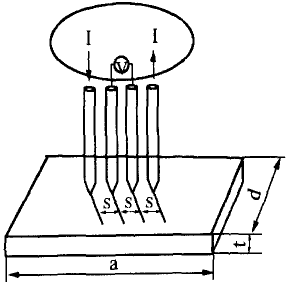
\includegraphics[scale = 0.5]{4probe.png}
    \caption{4 point probe measurement 모식도}
    \label{4probe}
  \end{figure}

시료가 얇은 경우(두께 $\ll$ 탐침 사이 간격), 시료의 두께를 $t$라 하면 면적 $A$는 
\begin{align}
    A = 2\pi xt
\end{align}
이고 저항 $R$은
\begin{align}
    R = \int_s^{2s} \rho\frac{1}{2\pi t}\frac{1}{x}\,dx =  \frac{\rho}{2\pi t}
    \ln{2}
\end{align}
이다. 옴의 법칙 $V=IR$에 의해 비저항 $\rho$는
\begin{align}
    \rho = \frac{\pi t}{\ln{2}}\frac{V}{I}
\end{align}
로 구할 수 있다. 


\subsection{Experimental Methods}
\subsubsection{For matter}
\begin{itemize}
    \item[1. ]
    4 point probe 장비와 Voltage meter, Current source를 연결선을 통해 연결한다.
    \item[2. ]
    4 point probe 장비와 Oven을 연결한다.
    \item[3. ]
    4 point probe의 샘플 스테이지에 시료를 놓는다. 이때, 4 point probe 장비에 
    적절한 압력을 주어 탐침과 시료가 닿도록 만들고, 나사를 조여 고정한다. 
    \item[4. ]
    Oven의 스위치를 set으로 올려주고 다이얼을 돌려 25℃로 설정해준다.
    \item[5. ]
    Current source와 Voltage meter의 스케일을 적절히 설정하고, 영점을 맞춘다.
    \item[6. ]
    Current source의 다이얼을 돌려 4 point probe의 전류를 증가시키며, 
    이에 따른 전압을 Voltage meter로 측정한다.
    \item[7. ] 
    측정한 전압과 전류 사이의 관계식을 사용하여 시료의 종류에 
    따른 비저항과 면저항을 계산한다. 
    \begin{align}
        \rho = \frac{\pi TV}{\ln{2I}}\approx 4.532\frac{TV}{I},\,\,\,
        \rho_s = \frac{\rho}{T}\approx 4.532\frac{V}{I}
    \end{align}

\end{itemize}


\subsubsection{For temperature}
\begin{itemize}
    \item[1. ]
    Oven의 스위치를 set으로 올려주고 다이얼을 돌려 원하는 값을 설정해준다.
    \item[2. ]
    설정한 값이 일정하게 유지되고 있는 지를 Display를 통해 확인한다. 
    \item[3. ]
    Current source의 다이얼을 조금씩 돌려가며 전류가 증가함에 따라 변화하는 전압을 
    Voltage meter로 측정한다. 
    \item[4. ]
    Oven의 다이얼을 돌려 기존의 값과 다른 온도를 설정해준다.
    \item[5. ]
    2~3번을 반복한다. 
    \item[6. ]
    전류와 전압 사이의 관계를 이용하여 온도에 따른 비저항을 구하고, 
    온도와 비저항이 어떤 관계를 가지는 지 분석한다.

\end{itemize}
\nocite{*} 
\bibliography{ref}



%\begin{thebibliography}{9}
%\end{thebibliography}

\vfill
\end{document}